%=========================================================
\chapter{Modelo del alcance}
\label{cap:reqUsr}

Este capítulo presenta el análisis detallado de la problemática operativa que enfrenta la Fundación Futuro con Derechos, los objetivos generales y específicos que guían el proyecto, el modelado y perfiles de los usuarios identificados en la organización, el mapa conceptual de los procesos afectados por la plataforma, la lista oficial de requerimientos de usuario y la especificación de la plataforma tecnológica del sistema \textbf{Taimotla}.

%---------------------------------------------------------
\section{Análisis de la problemática}

A continuación se expone el análisis del problema que sustenta el desarrollo del software. Este análisis describe las características de la operación actual de la Fundación para detallar los problemas identificados, sus causas, consecuencias y las características de la solución propuesta.

\subsection{Contexto del proyecto}

La \textbf{Fundación Futuro con Derechos} es una organización de la sociedad civil ubicada en el estado de Nuevo León que tiene como fin primordial la restitución de los derechos humanos y garantías constitucionales de niñas, niños y adolescentes (NNA) en estado de orfandad debido al feminicidio de sus madres. Para coordinar y dirigir la operación, la estructura organizacional cuenta con una Dirección General, que se apoya en una Coordinación Operativa para supervisar y gestionar a los equipos multidisciplinarios de caso.

Los equipos multidisciplinarios son células de trabajo de alto rendimiento compuestas por profesionales de cuatro especialidades clave: un psicólogo, un médico, un trabajador social y un abogado. Su propósito es realizar una valoración diagnóstica del menor y su entorno sociofamiliar, identificar vulneraciones a sus derechos y trazar conjuntamente un Plan de Restitución de Derechos (PRD) de manera coordinada. Este proceso de restitución se fundamenta jurídicamente en el artículo 123 de la Ley General de los Derechos de Niñas, Niños y Adolescentes (LGDNNA) y adopta metodológicamente los estándares promovidos en la Caja de Herramientas de la UNICEF y el Formulario Único de Datos (FUD).

Debido al incremento acelerado en la matrícula de casos activos en el estado de Nuevo León y al gran volumen de información clínica, legal, social y escolar que se genera por cada menor, la Fundación presenta graves dificultades en el control y resguardo de su información. La operación manual basada en archivos de texto locales, hojas de cálculo aisladas, copias físicas y canales de comunicación informales dificulta la coordinación de los especialistas, retrasa la consulta y pone en riesgo la seguridad de datos sumamente confidenciales de los menores.

\subsection{Problemas identificados}

El problema general que atiende este proyecto se define de la siguiente manera:

\begin{quote}
	{\em ``La gestión operativa e institucional de la Fundación está siendo rebasada por la dispersión, heterogeneidad y falta de estandarización en la información de los casos de NNA, generando retrasos en los tiempos de respuesta legal, vulnerabilidad ante la pérdida de datos altamente sensibles y lagunas temporales en el seguimiento continuo del proceso de restitución de derechos.''}
\end{quote}

Los problemas específicos identificados en la operación de la Fundación se detallan en la tabla~\ref{tbl:problemasIdentificados}:

\begin{problemas}
	
	\problema{P-01}{Heterogeneidad de datos}{La información de los expedientes está dispersa en múltiples soportes físicos y archivos locales (Word, notas sueltas, carpetas físicas), dificultando la integración y consulta rápida del caso.}{A}
	\problema{P-02}{Lentitud en la consulta de información}{El personal invierte tiempo excesivo en localizar documentos de identidad y salud del menor en carpetas físicas y discos locales de diferentes computadoras, lo que retrasa los trámites legales y médicos urgentes.}{A}
	\problema{P-03}{Vulnerabilidad y riesgo de pérdida de datos}{Almacenamiento local de la información en equipos individuales. Si un disco se daña, un equipo se extravía o un colaborador se retira de la fundación, se corre el riesgo de perder el historial completo de un menor de forma irreparable.}{MA}
	\problema{P-04}{Interrupción en el seguimiento de caso}{El seguimiento de la restitución de derechos no es continuo por falta de herramientas de control de fechas límite, provocando lagunas temporales sobre el estatus real de los derechos del menor.}{MA}
	\problema{P-05}{Inconsistencia de datos}{Falta de sincronización entre especialistas del mismo equipo. Por ejemplo, el médico puede actualizar un diagnóstico físico en un papel que el abogado o el psicólogo desconocen o no tienen registrado.}{M}
	\problema{P-06}{Sobrecarga operativa del personal}{El aumento acelerado de casos supera la capacidad del personal para redactar y consolidar reportes de manera manual, restando tiempo de atención directa a los menores.}{A}
	\problema{P-07}{Falta de personal capacitado en TIC}{La disparidad en las habilidades tecnológicas del personal operativo limita el aprovechamiento de herramientas informáticas genéricas, requiriendo un sistema intuitivo y adaptado a sus flujos de trabajo.}{M}
	\caption{Problemas identificados en la operación de la Fundación.}\label{tbl:problemasIdentificados}\\
\end{problemas}

\subsection{Análisis de causas probables}

\begin{description}
	\item[C-01 Uso de herramientas de almacenamiento descentralizadas:] El uso de carpetas locales, hojas de cálculo de Word/Excel y expedientes impresos impide la edición concurrente, el control de versiones y el respaldo automatizado de la información (Causa directa de P-01, P-02, P-03 y P-05).
	\item[C-02 Falta de una plataforma con flujos de trabajo centralizados:] La carencia de un sistema de notificaciones y recordatorios centralizados sobre plazos legales y médicos impide a los coordinadores y especialistas monitorear el avance de las medidas en tiempo real (Causa de P-04).
	\item[C-03 Inexistencia de un estándar operativo digitalizado:] Cada colaborador maneja su propio formato de trabajo y almacenamiento. Esto incrementa los tiempos de capacitación para el nuevo personal y genera cuellos de botella administrativos (Causa de P-06 y P-07).
\end{description}

\subsection{Análisis de posibles consecuencias}

\begin{description}
	\item[PC-01 Pérdida de la integridad y consistencia de los datos:] Existencia de información contradictoria en los expedientes de NNA, lo que inhabilita a la Fundación para entregar reportes confiables ante auditorías de la Procuraduría de Protección o dependencias gubernamentales (Consecuencia de P-01 y P-05).
	\item[PC- 02 Vulnerabilidad jurídica y física de los NNA:] Si un menor carece de su expediente unificado, se pueden aplicar medidas de protección incorrectas o tardías, categorizando casos como ``resueltos'' cuando no lo están, dejando desprotegido al menor ante su entorno de riesgo (Consecuencia de P-04).
	\item[PC - 03 Filtración de información altamente sensible:] El almacenamiento y envío desordenado de datos personales de menores víctimas de violencia puede derivar en fugas de información, poniendo en riesgo la integridad física del menor y de su red de apoyo familiar (Consecuencia de P-03).
	\item[PC - 04 Retrasos administrativos severos y pérdida de credibilidad:] Incapacidad de responder a tiempo ante requerimientos de juzgados familiares o fiscalías debido al desorden en la consulta del archivo (Consecuencia de P-02).
	\item[PC - 05 Afectación a la salud laboral del personal y deserción operativa:] La sobrecarga extrema provocada por la redacción manual de informes y la duplicidad de tareas mecánicas genera agotamiento crónico en los especialistas. Esto incrementa la probabilidad de errores humanos críticos en los diagnósticos y provoca una alta rotación de personal, lo que interrumpe la continuidad y la confianza en los procesos de atención directa de los menores (Consecuencia de P-06).
    \item[PC - 06 Incapacidad institucional ante el incremento de la demanda:] La falta de automatización en la consolidación de reportes satura los tiempos de la estructura multidisciplinaria. Al no poder procesar la información de forma ágil, la Fundación se enfrenta a la imposibilidad de absorber nuevos casos, dejando desatendidas a Niñas, Niños y Adolescentes que requieren incorporarse urgentemente a un Plan de Restitución de Derechos (Consecuencia de P-06).
    \item[PC - 07 Resistencia al uso del sistema y persistencia del error:] Si la plataforma tecnológica no se adapta intuitivamente a las capacidades reales de los usuarios, se generará frustración y un rechazo sistemático hacia la herramienta digital. Esto obligaría al personal a regresar al uso de formatos informales o registros manuales descentralizados, perpetuando el riesgo de extravío de información y las lagunas de datos en los expedientes (Consecuencia de P-07).
\end{description}

\subsection{Características de la solución}

Para mitigar la problemática de la Fundación, la solución de software propuesta debe cumplir con las siguientes características:
\begin{itemize}
	\item Estandarizar el registro y consulta de expedientes de NNA bajo una misma interfaz intuitiva.
	\item Centralizar los datos en un servidor seguro con base de datos relacional para evitar la fragmentación y pérdida de datos.
	\item Restringir los accesos a la información confidencial mediante roles definidos (Director, Coordinador, Especialista).
	\item Emitir notificaciones de plazos y tareas críticas para el seguimiento continuo de los planes de restitución.
	\item Que todos los documentos y reportes sean generados desde el sistema.
\end{itemize}

\subsection{Síntesis de la problemática}

En acuerdo con la Dirección General y la Coordinación Operativa de la Fundación, se han determinado las siguientes soluciones tecnológicas a implementar en el sistema \textbf{Taimotla}:

\begin{description}
	\item[S-01 Base de datos centralizada:] Implementación de una base de datos relacional a través del sistema gestor de bases de datos PostgreSQL único de donde se extraerá y sincronizará toda la información.
	\item[S-02 Autenticación y control de accesos basado en roles:] Limitación del acceso a los expedientes únicamente al equipo multidisciplinario responsable del caso y a la Dirección General.
	\item[S-03 Módulo de gestión de personal multidisciplinario:] Registro, actualización y control de estatus de los usuarios (activo/inactivo) realizado por el Coordinador.
	\item[S-04 Módulo de creación y gestión de equipos:] Asignación estructurada de un coordinador y especialistas a un expediente para asegurar responsables del seguimiento.
	\item[S-05 Formulario Único de Datos (FUD) digital:] Módulo de alta de NNA que captura de manera estandarizada los datos de identidad, etnia, nacionalidad, tutores e historial del hecho victimal.
	\item[S-06 Módulos específicos de especialidad:] Secciones especializadas en el expediente para que cada profesional (Médico, Psicólogo, Abogado, Trabajador Social) registre diagnósticos de su competencia.
	\item[S-07 Gestión y carga documental:] Módulo para subir, resguardar y validar actas de nacimiento y cartillas médicas digitalizadas.
	\item[S-08 Control de estatus del expediente:] Flujo de estados para el expediente del menor (Creado, En Diagnóstico, Plan Asignado, En Seguimiento, Cerrado).
	\item[S-09 Alertas visuales de plazos límite:] Semáforo de tiempos para notificar la fecha límite de vencimiento de las medidas de protección y evitar interrupciones de seguimiento.
	\item[S-10 Operación vía plataforma web:] Acceso mediante navegadores de escritorio estándar sin requerir instalación de software especializado en los equipos locales.
\end{description}

%---------------------------------------------------------
\section{Objetivos del proyecto}

\subsection{Objetivo general}

Desarrollar un sistema de información web centralizado para la gestión de expedientes digitales y la coordinación del equipo multidisciplinario, con el fin de optimizar el seguimiento continuo y garantizar la oportuna restitución de los derechos de las niñas, niños y adolescentes en estado de orfandad por femicidio atendidos por la Fundación Futuro con Derechos en el estado de Nuevo León.

\subsection{Objetivos específicos}

\begin{itemize}
	\item Centralizar y unificar los datos operativos, clínicos, sociofamiliares y jurídicos de los NNA en una base de datos relacional y segura, eliminando el uso de herramientas descentralizadas.
	\item Estandarizar el registro de la información de los casos mediante interfaces específicas basadas en la metodología FUD y la Caja de Herramientas de UNICEF.
	\item Implementar un control de accesos estricto basado en perfiles de usuario y roles operativos para resguardar la confidencialidad de la información confidencial de los menores.
	\item Desarrollar un módulo de gestión y asignación de equipos multidisciplinarios para definir de manera clara las responsabilidades de atención de cada caso.
	\item Incorporar un sistema de alertas visuales basadas en plazos límite para garantizar la continuidad y evitar lagunas temporales en el seguimiento del Plan de Restitución de Derechos.
\end{itemize}

%---------------------------------------------------------
\section{Usuarios identificados}

El sistema \textbf{Taimotla} interactúa directamente con los miembros del área operativa de la Fundación. En la figura~\ref{fig:organigramaFundacion} se presenta el organigrama operativo de la institución, que define los niveles de supervisión y coordinación técnica para el sistema.

\begin{figure}[htbp]
	\begin{center}
		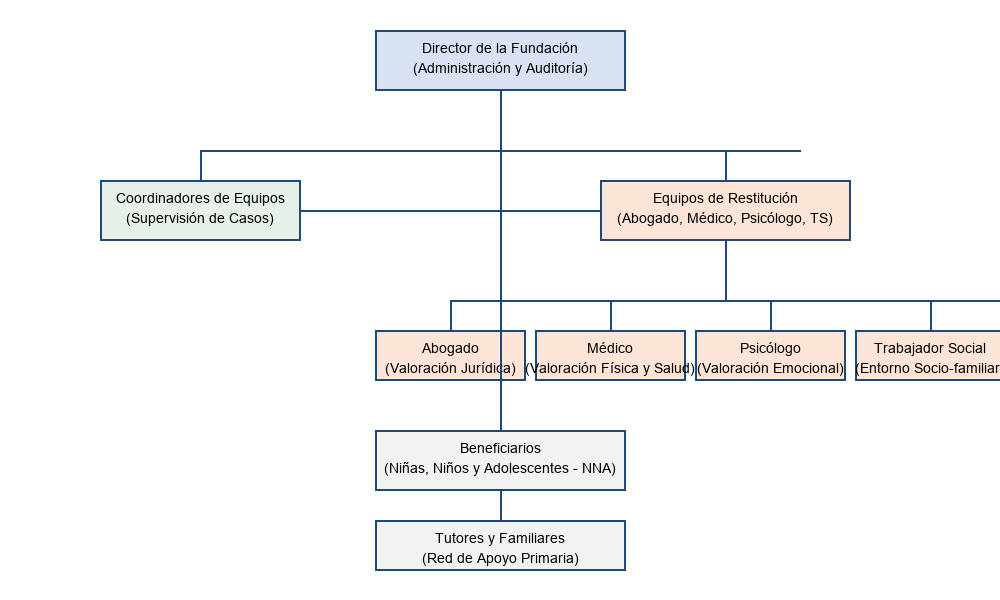
\includegraphics[width=.9\textwidth]{images/organigrama_fundacion}
		\caption{Estructura operativa de usuarios en la Fundación Futuro con Derechos.}
		\label{fig:organigramaFundacion}
	\end{center}
\end{figure}

A continuación, se detalla la jerarquía organizacional del área operativa en forma de organigrama y se define el perfil de cada uno de los actores identificados en el sistema:

\subsection{Perfil y Definición de Actores}

\subsubsection{Actor: Director de la Fundación}
\begin{description}
	\item[Descripción:] Es la máxima autoridad administrativa y operativa de la organización. Supervisa el desempeño global, gestiona el catálogo de personal y aprueba la formación de los equipos de trabajo.
	\item[Responsabilidades:] \cdtEmpty
		\begin{itemize}
			\item Registrar, actualizar, habilitar y deshabilitar las cuentas del personal multidisciplinario (coordinadores, abogados, médicos, psicólogos y trabajadores sociales).
			\item Crear, modificar y disolver los equipos multidisciplinarios de trabajo.
			\item Auditar periódicamente la carga de expedientes y supervisar el estatus general de los casos de restitución.
		\end{itemize}
	\item[Perfil:] \cdtEmpty
		\begin{itemize}
			\item Licenciatura terminada en Administración, Derecho o Ciencias Sociales.
			\item Experiencia mínima de 3 años en dirección de organizaciones sociales o gubernamentales de protección de menores.
			\item Habilidad en la toma de decisiones estratégicas, auditoría y gestión de personal.
		\end{itemize}
	\item[Procesos en los que participa:] PRS-02, PRP-01, PRP-03.
	\item[Área:] Dirección General.
	\item[Cantidad aproximada:] 1.
	\item[Horario de actividad:] Horario laboral de la Fundación.
\end{description}

\subsubsection{Actor: Coordinador de Caso}
\begin{description}
	\item[Descripción:] Es el profesional encargado de liderar uno o varios equipos multidisciplinarios asignados a expedientes de NNA. Actúa como enlace entre el personal técnico y la dirección.
	\item[Responsabilidades:] \cdtEmpty
		\begin{itemize}
			\item Supervisar las valoraciones individuales de cada especialista en su equipo.
			\item Consolidar el Plan de Restitución de Derechos (PRD) y someterlo a revisión.
			\item Gestionar y asignar actividades específicas del expediente al personal multidisciplinario.
			\item Solicitar a la dirección la adición o remoción de integrantes de su equipo de acuerdo con las necesidades del caso.
		\end{itemize}
	\item[Perfil:] \cdtEmpty
		\begin{itemize}
			\item Licenciatura en Psicología, Derecho, Trabajo Social o afín, con especialización en derechos de la infancia.
			\item Liderazgo, facilidad de palabra y capacidad para coordinar grupos multidisciplinarios.
		\end{itemize}
	\item[Procesos en los que participa:] PRC-03, PRC-05, PRC-08.
	\item[Área:] Coordinación Operativa.
	\item[Cantidad aproximada:] 1 o más.
	\item[Horario de actividad:] Horario laboral de la Fundación.
\end{description}

\subsubsection{Actor: Abogado (Personal Multidisciplinario)}
\begin{description}
	\item[Descripción:] Especialista legal responsable del análisis jurídico del caso del menor y de la promoción de recursos legales para garantizar sus derechos.
	\item[Responsabilidades:] \cdtEmpty
		\begin{itemize}
			\item Realizar la valoración jurídica inicial del NNA y documentarla en el expediente.
			\item Solicitar, tramitar y dar seguimiento a las medidas urgentes de protección ante el Ministerio Público y juzgados familiares.
			\item Cargar y validar la documentación legal digital del NNA (actas de nacimiento, actas de detención, etc.).
		\end{itemize}
	\item[Perfil:] \cdtEmpty
		\begin{itemize}
			\item Licenciatura en Derecho con cédula profesional vigente.
			\item Conocimiento sólido de la LGDNNA, procesos de lo familiar y derecho penal juvenil.
		\end{itemize}
	\item[Procesos en los que participa:] PRC-04, PRC-06, PRC-07.
	\item[Área:] Equipo Multidisciplinario - Legal.
	\item[Cantidad aproximada:] Variable (uno por equipo multidisciplinario).
	\item[Horario de actividad:] Horario laboral de la Fundación.
\end{description}

\subsubsection{Actor: Médico (Personal Multidisciplinario)}
\begin{description}
	\item[Descripción:] Profesional de la salud encargado de evaluar el estado físico de las NNA, detectar afectaciones orgánicas y coordinar su atención en el sector salud.
	\item[Responsabilidades:] \cdtEmpty
		\begin{itemize}
			\item Realizar valoraciones clínicas de ingreso y periódicas al menor.
			\item Integrar el historial clínico físico y digital en el expediente único de Taimotla.
			\item Gestionar la vinculación a instituciones de salud especializadas y verificar la vigencia de seguros médicos o cartillas de vacunación.
		\end{itemize}
	\item[Perfil:] \cdtEmpty
		\begin{itemize}
			\item Licenciatura en Medicina con cédula profesional vigente y deseable especialidad en Pediatría o salud infantil.
			\item Sensibilidad en el trato con infantes víctimas de violencia.
		\end{itemize}
	\item[Procesos en los que participa:] PRC-04, PRC-06, PRC-07.
	\item[Área:] Equipo Multidisciplinario - Salud.
	\item[Cantidad aproximada:] Variable (uno por equipo multidisciplinario).
	\item[Horario de actividad:] Horario laboral de la Fundación.
\end{description}

\subsubsection{Actor: Psicólogo (Personal Multidisciplinario)}
\begin{description}
	\item[Descripción:] Especialista en salud mental responsable del diagnóstico del estado psicológico del menor y de proveer contención emocional durante el proceso de restitución.
	\item[Responsabilidades:] \cdtEmpty
		\begin{itemize}
			\item Aplicar baterías de pruebas y entrevistas para diagnosticar el grado de afectación emocional y grado de negación de NNA y sus tutores.
			\item Redactar y adjuntar los dictámenes psicológicos periciales en el expediente digital.
			\item Brindar sesiones de terapia psicológica y preparar al NNA antes de participar en diligencias ministeriales o judiciales.
		\end{itemize}
	\item[Perfil:] \cdtEmpty
		\begin{itemize}
			\item Licenciatura en Psicología con cédula profesional.
			\item Enfoque terapéutico clínico infantil y capacitación en atención a trauma y abuso.
		\end{itemize}
	\item[Procesos en los que participa:] PRC-04, PRC-06.
	\item[Área:] Equipo Multidisciplinario - Psicología.
	\item[Cantidad aproximada:] Variable (uno por equipo multidisciplinario).
	\item[Horario de actividad:] Horario laboral de la Fundación.
\end{description}

\subsubsection{Actor: Trabajador Social (Personal Multidisciplinario)}
\begin{description}
	\item[Descripción:] Profesional encargado de investigar el entorno social, familiar y socioeconómico en el que se desenvuelve el menor para trazar su red de apoyo.
	\item[Responsabilidades:] \cdtEmpty
		\begin{itemize}
			\item Realizar visitas domiciliarias y entrevistas a tutores y familiares de las NNA.
			\item Elaborar los estudios socioeconómicos y reportes de entorno social.
			\item Identificar e informar sobre el patrón de migración, nivel educativo, escolaridad y ocupación del tutor o familiar directo.
		\end{itemize}
	\item[Perfil:] \cdtEmpty
		\begin{itemize}
			\item Licenciatura en Trabajo Social con cédula profesional.
			\item Capacidad de análisis de entornos vulnerables, empatía y técnicas de entrevista familiar.
		\end{itemize}
	\item[Procesos en los que participa:] PRC-04, PRC-08.
	\item[Área:] Equipo Multidisciplinario - Trabajo Social.
	\item[Cantidad aproximada:] Variable (uno por equipo multidisciplinario).
	\item[Horario de actividad:] Horario laboral de la Fundación.
\end{description}


%---------------------------------------------------------
\section{Procesos involucrados}

Al digitalizar las operaciones de la Fundación mediante \textbf{Taimotla}, los procesos tradicionales se automatizarán y centralizarán. A continuación se define el mapa de procesos de la organización, clasificándolos en procesos estratégicos, clave y de soporte:

\subsection{Clasificación de Procesos}

\subsubsection{Procesos Estratégicos}
\begin{description}
	\item[PRS-02 * Supervisión y Auditoría de Casos:] Monitoreo del estado y avance de los expedientes por parte del Director de la Fundación para garantizar el apego a los plazos legales del artículo 123 de la LGDNNA.
\end{description}

\subsubsection{Procesos Clave}
\begin{description}
	\item[PRC-01 Recepción y Detección de Casos:] Detección o canalización inicial del caso del menor que se encuentra en situación de orfandad por feminicidio.
	\item[PRC-02 * Registro de NNA y Apertura de Expediente:] Alta del menor en la base de datos centralizada del sistema, capturando su CURP, nacionalidad, etnia, datos de contacto e identidad básica.
	\item[PRC-03 * Asignación de Equipo Responsable:] Formación de un equipo de trabajo (compuesto por un coordinador y entre 2 y 4 especialistas multidisciplinarios) para encargarse de forma exclusiva de la atención del expediente del NNA.
	\item[PRC-04 * Valoración y Diagnóstico Multidisciplinario:] Registro digital de los diagnósticos iniciales del menor en materia clínica, psicológica, socio-familiar y jurídica.
	\item[PRC-05 * Elaboración del Plan de Restitución - PRD:] Registro y estructuración de los derechos vulnerados detectados (educación, salud, identidad) y las medidas recomendadas bajo el principio del interés superior del menor.
	\item[PRC-06 * Ejecución de Medidas Especiales y Urgentes:] Control de las solicitudes y estatus de ejecución de medidas de protección (ej. acogimiento residencial, terapia de contención, cirugías, trámites legales).
	\item[PRC-07 * Carga y Gestión Documental:] Carga digitalizada al servidor del sistema de los documentos comprobatorios obligatorios del menor (acta de nacimiento, cartilla de vacunación, CURP, etc.) con sus metadatos y vigencias.
	\item[PRC-08 * Seguimiento de Restitución:] Consultas periódicas sobre la restitución de cada uno de los derechos del NNA.
	\item[PRC-09 * Cierre de Expediente:] Archivo histórico y conclusión del caso tras validar que todos los derechos de la NNA han sido plenamente garantizados.
\end{description}

\subsubsection{Procesos de Soporte}
\begin{description}
	\item[PRP-01 * Gestión de Personal Multidisciplinario:] Registro, edición de perfil, desactivación (deshabilitado) y reactivación (habilitado) de las credenciales de los empleados del sistema.
	\item[PRP-02 * Control de Accesos y Seguridad:] Control de sesiones de usuario (Director, Coordinadores y personal) con contraseñas seguras y restricciones de rol.
	\item[PRP-03 * Mantenimiento de Catálogos:] Actualización en la base de datos de catálogos paramétricos requeridos por el sistema (tales como sexos, etnias, nacionalidades, tipos de documentos, parentescos, etc.).
\end{description}


%---------------------------------------------------------
\section{Requerimientos de usuario}

Los requerimientos de usuario extraídos de la operación de la Fundación se especifican en la tabla~\ref{tbl:requerimientosUsuario}:

\begin{requerimientosU}
	
	\FRitem{RU-01}{Consulta de casos asignados}{El personal necesita consultar los casos que tiene asignados.}{1}{\TODO}
	\FRitem{RU-02}{Seguimiento del estado del caso}{El personal necesita saber en qué estado se encuentra cada caso de NNA que atiende.}{1}{\TODO}
	\FRitem{RU-03}{Registro del NNA}{El personal necesita registrar a los NNA que ingresan a la Fundación.}{1}{\TODO}
	\FRitem{RU-04}{Asignación de casos a equipos}{El Coordinador necesita asignar los casos de NNA a los equipos multidisciplinarios.}{1}{\TODO}
	\FRitem{RU-05}{Gestión de equipos multidisciplinarios}{El Coordinador necesita conformar y gestionar los equipos multidisciplinarios.}{1}{\TODO}
	\FRitem{RU-06}{Gestión del personal de la Fundación}{El Director necesita registrar y administrar las cuentas del personal.}{2}{\TODO}
	\FRitem{RU-07}{Carga de documentos del NNA}{El personal necesita adjuntar los documentos oficiales del NNA al expediente.}{2}{\TODO}
	\FRitem{RU-08}{Registro del entorno familiar del NNA}{El Trabajador Social necesita registrar la información del entorno familiar del NNA.}{2}{\TODO}
	\FRitem{RU-09}{Registro del tutor o cuidador del NNA}{El personal necesita registrar los datos del tutor o cuidador responsable del NNA.}{2}{\TODO}
	\FRitem{RU-10}{Registro del historial médico del NNA}{El Médico necesita registrar el historial clínico y el esquema de vacunación del NNA.}{2}{\TODO}
	\FRitem{RU-11}{Registro del hecho victimal}{El personal necesita documentar el hecho que originó la vulneración de derechos del NNA.}{2}{\TODO}
	\FRitem{RU-12}{Mantenimiento de catálogos del sistema}{El Director necesita mantener actualizados los catálogos de valores del sistema.}{2}{\TODO}
	\FRitem{RU-13}{Diagnóstico clínico del NNA}{El Médico necesita registrar el diagnóstico clínico inicial del NNA.}{4}{\TODO}
	\FRitem{RU-14}{Diagnóstico psicológico del NNA}{El Psicólogo necesita registrar el diagnóstico del estado emocional del NNA.}{4}{\TODO}
	\FRitem{RU-15}{Diagnóstico jurídico del NNA}{El Abogado necesita registrar la valoración jurídica del caso del NNA.}{4}{\TODO}
	\FRitem{RU-16}{Diagnóstico sociofamiliar del NNA}{El Trabajador Social necesita registrar el diagnóstico del entorno social del NNA.}{4}{\TODO}
	\FRitem{RU-17}{Identificación de derechos vulnerados}{El Coordinador necesita registrar qué derechos del NNA han sido vulnerados.}{4}{\TODO}
	\FRitem{RU-18}{Plan de Restitución de Derechos}{El Coordinador necesita elaborar el Plan de Restitución de Derechos del NNA.}{4}{\TODO}
	\FRitem{RU-19}{Registro de medidas urgentes}{El Coordinador necesita registrar las medidas urgentes de protección solicitadas.}{4}{\TODO}
	\FRitem{RU-20}{Seguimiento de medidas de protección}{El personal necesita registrar el avance de cada medida de protección del plan.}{4}{\TODO}
	\FRitem{RU-21}{Catálogo de actores en materia de derechos}{El personal necesita consultar las organizaciones y personas que pueden apoyar la restitución de derechos del NNA.}{4}{\TODO}
	\FRitem{RU-22}{Gestión de actores en materia de derechos}{El Coordinador necesita registrar y actualizar la información de los actores en materia de derechos.}{4}{\TODO}
	\FRitem{RU-23}{Vinculación de actores al plan}{El Coordinador necesita asociar actores responsables a cada medida del plan.}{4}{\TODO}
	\FRitem{RU-24}{Familiograma del NNA}{El Trabajador Social necesita construir el familiograma del NNA.}{4}{\TODO}
	\FRitem{RU-25}{Alertas de fechas importantes}{El personal necesita recibir alertas cuando se acercan fechas límite de los casos.}{4}{\TODO}
	\FRitem{RU-26}{Cierre del expediente}{El Coordinador necesita registrar el cierre del caso cuando todos los derechos han sido restituidos.}{4}{\TODO}
	\FRitem{RU-27}{Historial del expediente}{El personal necesita consultar el historial completo de acciones realizadas en un caso.}{4}{\TODO}
	\FRitem{RU-28}{Supervisión general de casos}{El Director necesita una vista general del estado de todos los expedientes activos.}{4}{\TODO}
	\caption{Requerimientos de usuario del sistema Taimotla.}\label{tbl:requerimientosUsuario}\\
\end{requerimientosU}

%---------------------------------------------------------
\section{Requerimientos funcionales}

Los requerimientos funcionales del sistema Taimotla, que detallan las funciones de la plataforma tecnológica y su trazabilidad con las necesidades de usuario, se especifican en la tabla~\ref{tbl:requerimientosFuncionales}:

\begin{requerimientos}
	
	\FRitem{RF-01}{Autenticación de usuarios}{El sistema debe permitir a los colaboradores iniciar sesión ingresando su correo institucional y contraseña.}{A}{RU-01}
	\FRitem{RF-02}{Cierre de sesión}{El sistema debe permitir a los usuarios finalizar su sesión activa y destruir las variables de sesión locales.}{M}{RU-01}
	\FRitem{RF-03}{Recuperación de contraseña}{El sistema debe permitir a los usuarios recuperar sus accesos mediante el envío de un enlace al correo registrado.}{M}{RU-01}
	\FRitem{RF-04}{Registro de personal}{El sistema debe permitir al Director registrar cuentas de nuevos colaboradores del equipo multidisciplinario.}{A}{RU-08}
	\FRitem{RF-05}{Modificación de personal}{El sistema debe permitir al Director actualizar el perfil, rol y la especialidad de los empleados registrados.}{M}{RU-08}
	\FRitem{RF-06}{Habilitación de cuentas}{El sistema debe permitir al Director cambiar el estado de la cuenta (activo/inactivo) para dar de baja accesos.}{A}{RU-08}
	\FRitem{RF-07}{Registro de NNA (FUD)}{El sistema debe permitir capturar los datos generales de la NNA (CURP, nombre, apodo, etnia, nacionalidad, escolaridad).}{A}{RU-03}
	\FRitem{RF-08}{Registro de red familiar}{El sistema debe permitir registrar los datos de contacto, ocupación y parentesco de los tutores de la NNA.}{A}{RU-03}
	\FRitem{RF-09}{Registro de hecho victimal}{El sistema debe permitir capturar el reporte, fecha de detención, relato de hechos y nombre de la madre víctima.}{A}{RU-03}
	\FRitem{RF-10}{Consulta de expedientes}{El sistema debe permitir consultar en un panel unificado los datos FUD, documentos y valoraciones del menor.}{A}{RU-02}
	\FRitem{RF-11}{Captura de valoraciones}{El sistema debe permitir a los especialistas capturar notas y diagnósticos en las pestañas correspondientes a su área.}{A}{RU-04}
	\FRitem{RF-12}{Carga digital de documentos}{El sistema debe permitir al personal digitalizar y cargar actas de nacimiento y cartillas de salud en PDF/JPG/PNG.}{A}{RU-09}
	\FRitem{RF-13}{Asignación de expedientes}{El sistema debe permitir al Coordinador de Caso vincular un expediente abierto a un equipo de especialistas.}{A}{RU-05}
	\FRitem{RF-14}{Seguridad por rol y caso}{El sistema debe restringir la edición del expediente únicamente a los miembros del equipo multidisciplinario asignado.}{A}{RU-07}
	\FRitem{RF-15}{Alertas de plazos límite}{El sistema debe emitir alertas visuales de tiempos y vigencias para el vencimiento de las medidas del PRD.}{A}{RU-03}
	\FRitem{RF-16}{Búsqueda dinámica de NNA}{El sistema debe permitir realizar búsquedas en tiempo real de expedientes de menores por nombre o CURP para agilizar la consulta.}{A}{RU-02}
	\FRitem{RF-17}{Modificación de expediente de NNA}{El sistema debe permitir actualizar la información previamente capturada en cualquiera de las secciones del expediente unificado.}{A}{RU-03}
	\FRitem{RF-18}{Creación de equipos}{El sistema debe permitir al Director conformar nuevos equipos multidisciplinarios asignándoles un nombre, un coordinador y vinculando hasta 4 especialistas disponibles.}{A}{RU-06}
	\FRitem{RF-19}{Edición de equipos de trabajo}{El sistema debe permitir al Director actualizar la composición de un equipo activo cambiando su coordinador, retirando integrantes o agregando nuevos especialistas en línea.}{M}{RU-06}
	\FRitem{RF-20}{Disolución de equipos}{El sistema debe permitir al Director eliminar de forma lógica un equipo registrado, liberando a sus integrantes y finalizando su participación actual.}{M}{RU-06}
	\FRitem{RF-21}{Eliminación permanente de cuentas}{El sistema debe permitir al Director eliminar de forma permanente la cuenta de un colaborador del sistema.}{M}{RU-08}
	\FRitem{RF-22}{Consulta de datos de cuenta propia}{El sistema debe permitir a los usuarios logueados consultar la información administrativa de su propia cuenta de acceso.}{M}{RU-01}
	\FRitem{RF-23}{Validación de acta de nacimiento}{El sistema debe permitir al Abogado marcar el acta de nacimiento de un NNA como verificada tras validar su autenticidad.}{A}{RU-09}
	\caption{Requerimientos funcionales del sistema Taimotla.}\label{tbl:requerimientosFuncionales}\\
\end{requerimientos}
	

%---------------------------------------------------------
\section{Especificación de plataforma}

El sistema web \textbf{Taimotla} se ha especificado para operar de forma centralizada bajo una arquitectura cliente-servidor estándar accesible vía navegador.

\begin{description}
	\item[Tipo de sistema:] Aplicación Web responsiva de gestión y base de datos relacional.
	\item[Software del cliente:] Navegadores modernos compatibles con HTML5 y CSS3 (Google Chrome, Mozilla Firefox, Microsoft Edge, Safari) ejecutándose sobre sistemas de escritorio o móviles.
	\item[Tecnología del servidor:] 
		\begin{itemize}
			\item Backend: Servidor con Python 3.x y microframework Flask.
			\item Base de datos: Sistema Gestor de Bases de Datos Relacionales (SGBD) PostgreSQL.
			\item Frontend: HTML5, Bootstrap 5, Vanilla CSS3 y JavaScript para micro-interacciones.
		\end{itemize}
	\item[Servicios requeridos:]
		\begin{itemize}
			\item Conexión cifrada a internet o red local (HTTP/HTTPS).
			\item Servicio de respaldo (backup) automatizado y periódico de la base de datos PostgreSQL.
			\item Control de sesiones web seguras mediante claves hash y variables de entorno cifradas.
		\end{itemize}
\end{description}
